\documentclass[12pt]{exam}
%\documentclass[12pt]{article}
\usepackage[letterpaper, margin=0.75in]{geometry}
\usepackage{graphicx}
\usepackage{enumitem}
\usepackage{booktabs}
\usepackage{amsmath}
\usepackage{tabularx}
\usepackage{color}

\begin{document}
\footer{}{Page \thepage\ of \numpages}{}

\begin{center}

\includegraphics[width=10cm]{../images/logo.png}
\end{center}

\begin{center}
\noindent{\LARGE Conceptual Physics \\ Class 14 Questions \\ May 11th, 2018  \\ ~ \\  Practice Questions for Second Partial Test \\ SOLUTIONS \\}
\end{center}

\vspace{0.2in}


\clearpage

\begin{questions}
\question Four point charges are arranged in 2 different configurations, resulting in different electric fields. Assume that the size of all charges are the same, and consider only the fact that some are positive and others are negative.

\begin{parts}

\part Draw the \textbf{electric} field lines around the following:
\vspace{0.25in}
\begin{center}
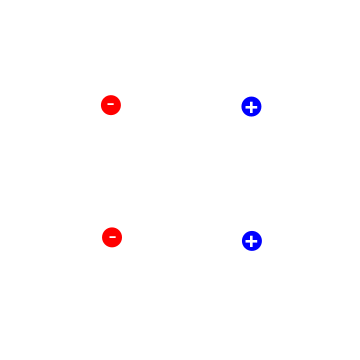
\includegraphics[width=3in]{../images/4chargesA.png}
\end{center}
\vspace{0.25in}

\part  Draw the \textbf{electric} field lines around the following:
\vspace{0.25in}
\begin{center}
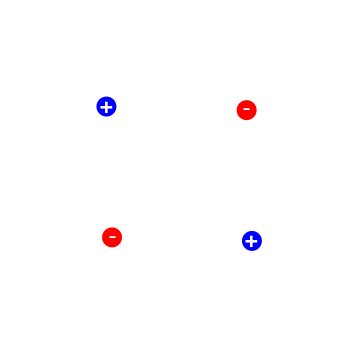
\includegraphics[width=3in]{../images/4chargesB.png}
\end{center}
\vspace{0.25in}

\clearpage
\part Draw the \textbf{gravitational} field lines around the following:
\vspace{0.25in}
\begin{center}
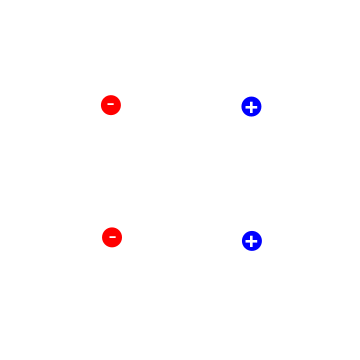
\includegraphics[width=3in]{../images/4chargesA.png}
\end{center}
\vspace{0.25in}

\part  Draw the \textbf{gravitational} field lines around the following:
\vspace{0.25in}
\begin{center}
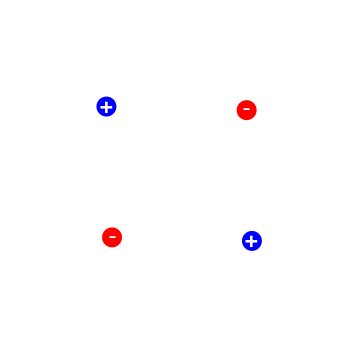
\includegraphics[width=3in]{../images/4chargesB.png}
\end{center}
\vspace{0.25in}
\end{parts}

\clearpage
\question Astronauts on three different spaceships are communicating with each other. Those aboard ships A and B agree on the rate at which time is passing, but they disagree with the people on ship C.

From \textit{Light and Matter,} Chapter 23 Question 3
\begin{parts}
	\part Alice is aboard ship A. How does she describe the motion of her own ship, in its frame of reference? (i.e. is it moving, not moving?)
		\begin{TheSolution}
			She does not think her own ship is moving.
		\end{TheSolution}
	\part Describe the motion of the other two ships, according to Alice. (Is ship B moving according to her? What about C?)
		\begin{TheSolution}
			\textbf{C is moving, B is not.} Since A and B agree on the passage of time, they must be stationary with respect to each other. Since A and C disagree on the passage of time, they must be moving with respect to each other.
		\end{TheSolution}
	\part Betty is in ship B. How does she describe the motion of her own ship, it its frame of reference?
		\begin{TheSolution}
			She does not think her own ship is moving.
		\end{TheSolution}
	\part Describe the motion of the other two ships, according to Betty. (Is ship A moving according to her? What about ship C?)
		\begin{TheSolution}
			\textbf{C is moving, A is not.} Since A and B agree on the passage of time, they must be stationary with respect to each other. Since B and C disagree on the passage of time, they must be moving with respect to each other.
		\end{TheSolution}
	\part Cathy is on ship C. How does she describe the motion of her own ship (C)? How would she describe the motion of ship A? Of ship B?
		\begin{TheSolution}
			\textbf{A and B are moving, C is not.} She does not this her own ship is moving, and since she disagrees on the passage of time with both A and B she must be moving with respect to them.
		\end{TheSolution}
\end{parts}

\question You can't use a light wave to see things that are smaller than the wavelength of the light.
\begin{parts}
	\part Using the diagram of the EM spectrum (on page 2 of this packet, or in your notes), what kind of light (radio, microwave, etc.) can be used to image atoms?
		\begin{TheSolution}
			x-rays and gamma rays, since their wavelengths are the same or smaller than that of an atom.
		\end{TheSolution}
	\part Using the diagram of the EM spectrum, what kind of light cannot be used to image atoms?
		\begin{TheSolution}
			Radio waves, microwaves, sub mm, infrared, visible and ultraviolet rays cannot be use to image atoms, since their wavelengths are much longer than the size of an atom.
		\end{TheSolution}
\end{parts}

\question A train is moving past a platform at a velocity $v$. Lightning bolts strike the front and back of the train, scorching both the train and the platform, as the train passes the platform. An observer at rest on the platform says the strikes were simultaneous. (Hint: For this problem, it may be easiest to draw diagrams on the extra scratch paper.)
\begin{center}
	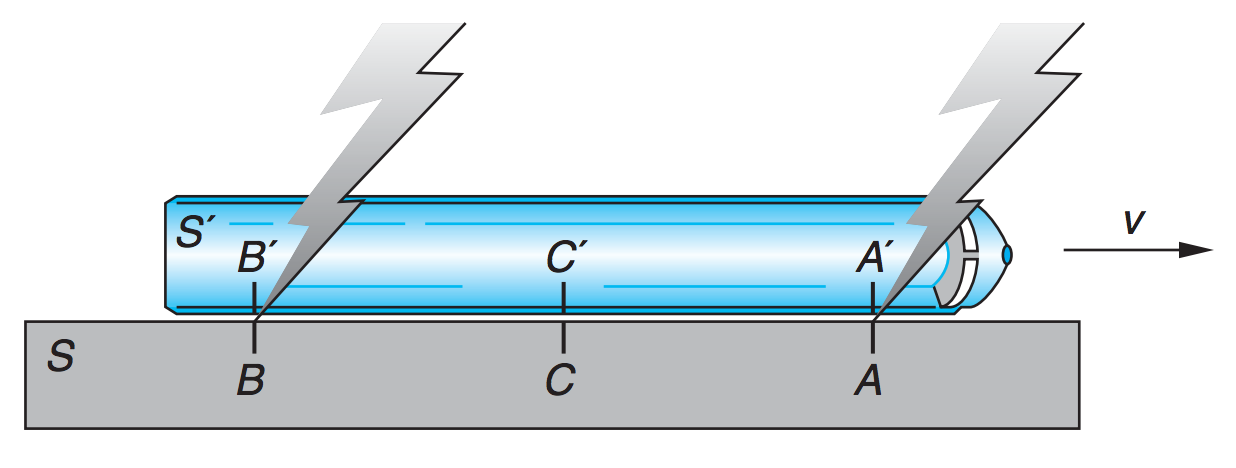
\includegraphics[width=0.7\textwidth]{../images/test2_lightning.png}
	\end{center}
	
	\begin{parts}
		\part A person on the platform says that the distance between \textit{scorched marks on the platform} is \textit{D}. To a person on the train, the distance between \textit{scorch marks on the platform} is:
		\begin{choices}
			\choice Longer than \textit{D}.
			\choice Shorter than \textit{D}.
			\choice Exactly \textit{D}.
			\choice Cannot say, we need more information.
		\end{choices}
		\begin{TheSolution}
			\textbf{B.} To a person on the train, they are stationary and the platform is moving. The platform is therefore length-contracted, and so they would see it as less than \textit{D}.
		\end{TheSolution}
		\part A person in the train measures the length of the train to be \textit{L}. To a person on the platform, is the train:
		\begin{choices}
			\choice Longer than \textit{L}.
			\choice Shorter than \textit{L}.
			\choice Exactly \textit{L}.
			\choice Cannot say, we need more information.
		\end{choices}
		\begin{TheSolution}
			\textbf{B.} To a person on the platform, they are stationary and the train is moving. The train is therefore length-contracted, and so they would see it as less than \textit{L}.
		\end{TheSolution}
		\part A person on the platform say that the distance between the \textit{scorch marks on the train} is also \textit{D} (since they see the strikes as happening at the same time). To a person on the train, the distance between \textit{scorch marks on the train} is:
		\begin{choices}
			\choice Longer than \textit{D}.
			\choice Shorter than \textit{D}.
			\choice Exactly \textit{D}.
			\choice Cannot say, we need more information.
		\end{choices}
		\begin{TheSolution}
			\textbf{A.} To a person on the platform, the train is length contracted and so appears shorter than it does to a person on the train: this is true for all measured lengths along the train. They would therefore see the distance between train scorch marks as shorter than a person on the train. Conversely a person on the train sees the train scorch marks as longer than would a person on the platform.
		\end{TheSolution}
		\part A person on the platform says the two strikes were simultaneous. What would a person on the train say?
		\begin{choices}
			\choice They would agree, the strikes happened simultaneously.
			\choice They would disagree, and say that the strike at \textit{A'} occurred before the strike at \textit{B'}
			\choice They would disagree, and say that the strike at \textit{B'} occurred before the strike at \textit{A'}
			\choice Cannot say, it is impossible for the person on the train to determine the order the strikes occurred.
		\end{choices}
		\begin{TheSolution}
			\textbf{B.} To a person on the train, the distance between scorch marks on the platform is less than \textit{D}, whereas the distance between scorch marks on the train is greater than \textit{D}. In order for this to occur, lighting would need to strike \textit{A'} before \textit{B'.}
		\end{TheSolution}
	\end{parts}

\question Three electrons have different energies. Using the ideas of wave/particle duality, we can represent the electrons as waves. The following images shows what their wavelength looks like:

\begin{center}
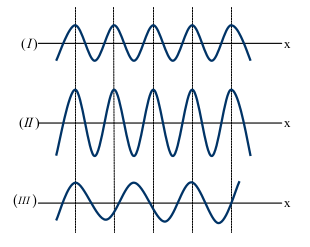
\includegraphics[width=4in]{../images/deBroglie.png}
\end{center}

The following questions will ask about how their energies, $E_I$, $E_{II}$, and $E_{III}$, relate.

\begin{parts}
	\part How do $E_I$ and $E_{II}$ compare?
		\begin{choices}
			\choice $E_{I} = E_{II}$
			\choice $E_{I} > E_{II}$
			\choice $E_{I} < E_{II}$
		\end{choices}
		\begin{TheSolution}
		\textbf{A.} Since the wavelength of the two are the same, the energies need to be the same.
		\end{TheSolution}
		\part How do $E_I$ and $E_{III}$ compare?
		\begin{choices}
			\choice $E_{I} = E_{III}$
			\choice $E_{I} > E_{III}$
			\choice $E_{I} < E_{III}$
		\end{choices}
		\begin{TheSolution}
			\textbf{B.} Since the wavelength of I is smaller than the wavelength at II, it must have a greater energy.
		\end{TheSolution}
	\part How do $E_{II}$ and $E_{III}$ compare?
		\begin{choices}
			\choice $E_{II} = E_{III}$
			\choice $E_{II} > E_{III}$
			\choice $E_{II} < E_{III}$
		\end{choices}
		\begin{TheSolution}
			\textbf{B.} Since the wavelength of II is smaller than the wavelength of III, it must have the greater energy.
		\end{TheSolution}
\end{parts}
	
	\question  You have a jar with 6 red balls and 4 green balls.
\begin{parts}
\part What is the probability of randomly drawing a red ball? What is the probability of randomly drawing a green ball?
\begin{TheSolution}
$P(\texttt{red}) = 6/10 = 0.6$, $P(\texttt{green}) = 4/10 = 0.4$. 
\end{TheSolution}
\part You randomly draw one ball, put it back, and draw a ball again. What is the probability of drawing a red and a green ball, in no particular order?
\begin{TheSolution}
There are two ways to do this: draw a red ball then a green ball, or draw a green ball then a red ball. $P(\texttt{red then green}) = 0.6\cdot 0.4 = 0.24$, $P(\texttt{green then red}) = 0.4\cdot 0.6 = 0.24$, so the probability of one or the other happening is 0.24 + 0.24 = 0.48.
\end{TheSolution}
\part You randomly draw one ball then draw another without putting back the first. What is the probability of drawing two red balls?
\begin{TheSolution}
On the first draw your probability of drawing red is 0.6. After drawing one red ball without replacement, your probability of drawing another red ball is 5/9, so your probability of drawing two red balls this way is $\frac{6}{10}\cdot\frac{5}{9} = 1/3$.
\end{TheSolution}
\part You randomly draw one ball then draw another without putting back the first. What is the probability of drawing a red and a green ball, in no particular order?
\begin{TheSolution}
There are two ways of doing this. One is to draw a red ball then a green ball; in this case, after drawing a red ball, your probability of drawing a green ball is 4/9, so $P(\texttt{red then green, no replacement}) = \frac{6}{10}\cdot\frac{4}{9} = \frac{24}{90} = \frac{4}{15}$. The other way is to draw a green ball then a red ball; in this case, after drawing a green ball, your probability of drawing a red ball is 6/9, so $P(\texttt{green then red, no replacement}) = \frac{4}{10}\cdot\frac{6}{9} = \frac{4}{15}$. The probability of either sequence of events happening is then 4/15 + 4/15 = 8/15.
\end{TheSolution}
\end{parts}

\question Consider the following experimental setups. Light of a given wavelength is incident on one of two  metal plates sealed inside a vacuum tube. The two plates are connected in circuit to an ammeter, a device that measures electric current. The metal plates have been thoroughly cleaned so that when blue light ($\lambda = 450$~nm) is incident on the lower plate, electrons are ejected.
\begin{parts}
\part There are two lightbulbs, which emit light at 300 nm and 400 nm. These wavelengths are shorter than blue light. Is the energy of the photons emitted by these two lightbulbs:
	\begin{choices}
		\choice The same as the energy contained in blue light (with wavelength 450 nm).
		\choice Greater than the energy contained in a blue light (with wavelength 450 nm).
		\choice Less than the energy contained in a blue light (with wavelength 450 nm).
	\end{choices}
	\begin{TheSolution}
	\textbf{B.} Since the wavelengths are both smaller than blue light, they have higher energy.
	\end{TheSolution}
\part In the following two setups, light of 300 nm and 400 nm wavelength (ultraviolet light) is incident on the lower plates. The number of photons landing on the metal plate per second is the same in both setups (they have the same intensity). Compare the number and energy of emitted electrons in the two setups.
\begin{center}
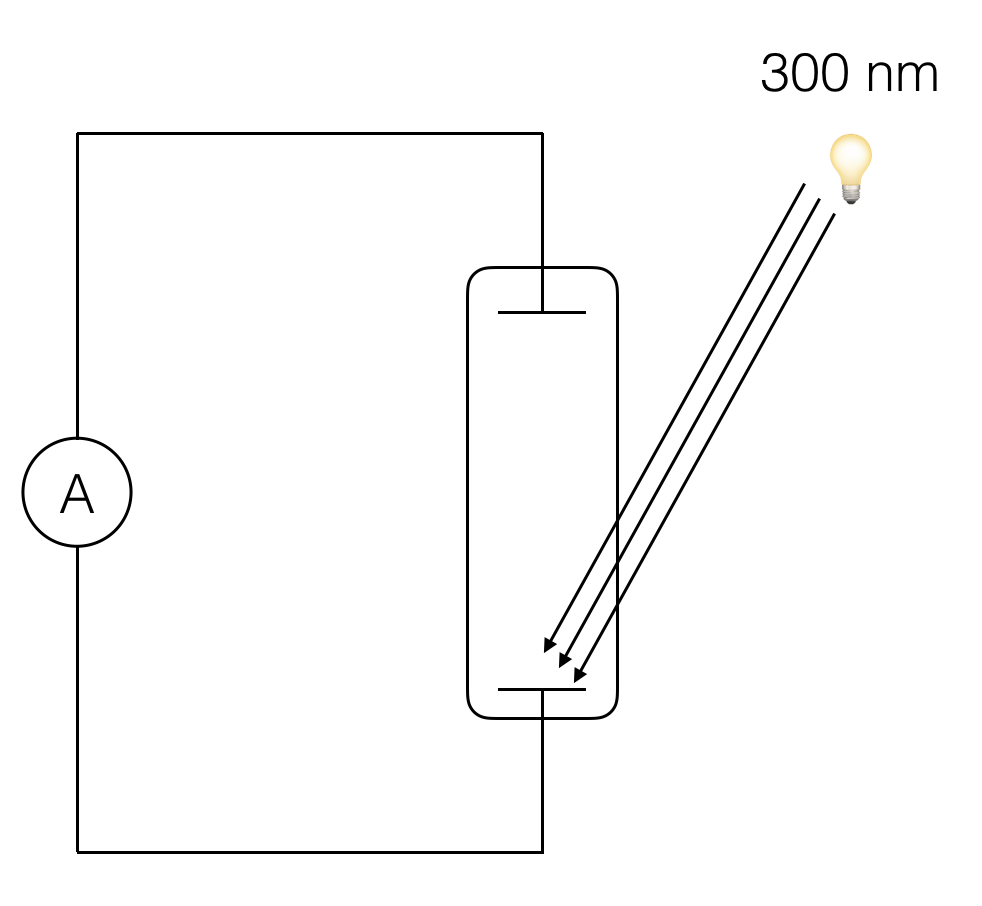
\includegraphics[width=0.45\textwidth]{../images/test2_300nm.png} 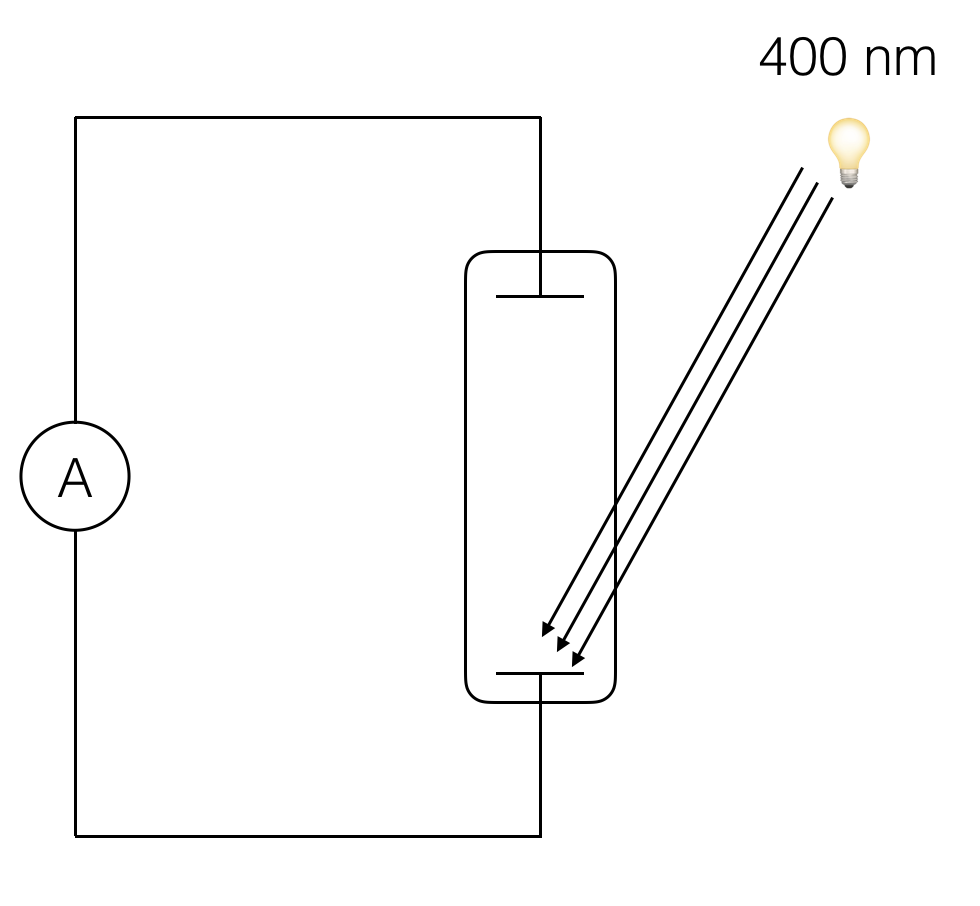
\includegraphics[width=0.45\textwidth]{../images/test2_400nm.png}
\end{center}
	\begin{choices}
		\choice The two setups emit the same number of electrons, however the setup on the left emits electrons with greater energies.
		\choice The two setups emit the same number of electron, however the setup on the right emits electrons with greater energies.
		\choice The two setups emit electrons at the same energies, however the setup on the left emits more.
		\choice The two setups emit electrons at the same energies, however the setup on the right emits more.
		\choice The two setups emit the same number of electrons and at the same energies.
	\end{choices}
	\begin{TheSolution}
		\textbf{A.} Since the intensities are the same, the number of emitted electrons is the same in both setups. However, since light on the left has a shorter wavelength than the light on the right, it has more energy and thus transfers more energy to the electrons.
	\end{TheSolution}

\part In the following two setups, light of 300 nm wavelength (ultraviolet light) is incident on the lower plates. There are three times as many photons landing on the metal plate per second in the setup on the left (the left light has a greater intensity). Compare the number and energy of emitted electrons in the two setups.
\begin{center}
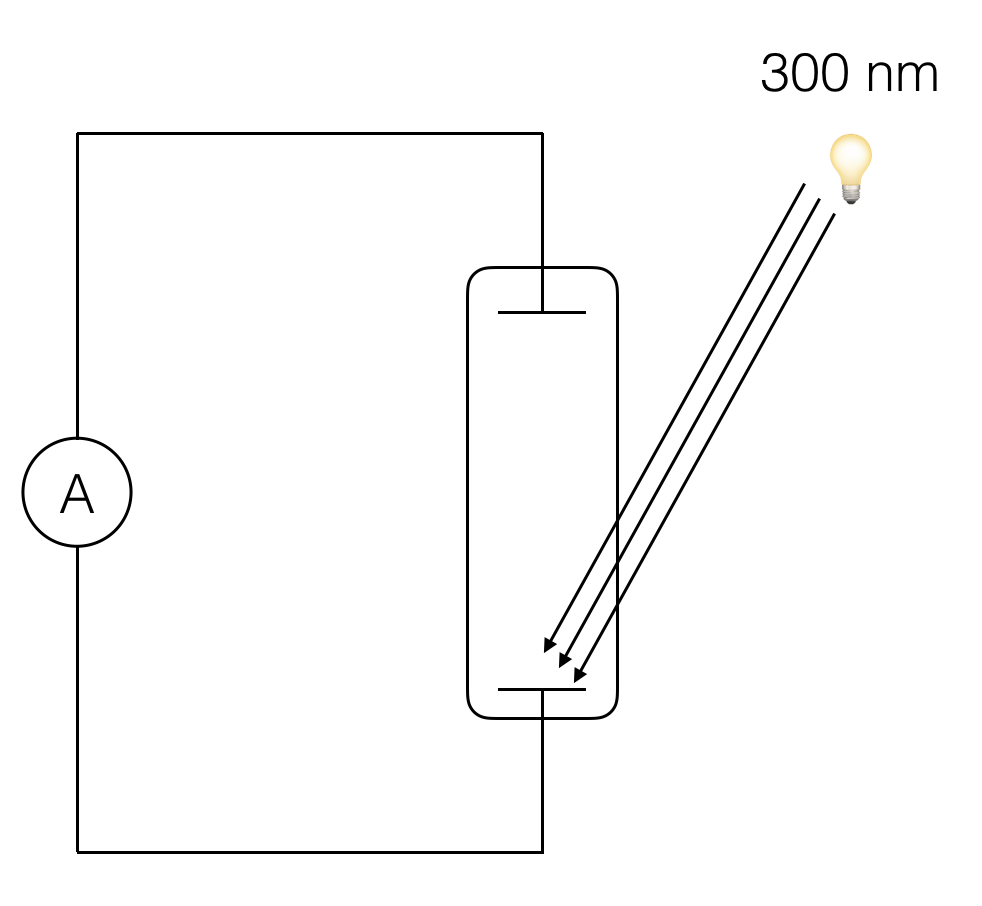
\includegraphics[width=0.45\textwidth]{../images/test2_300nm.png} 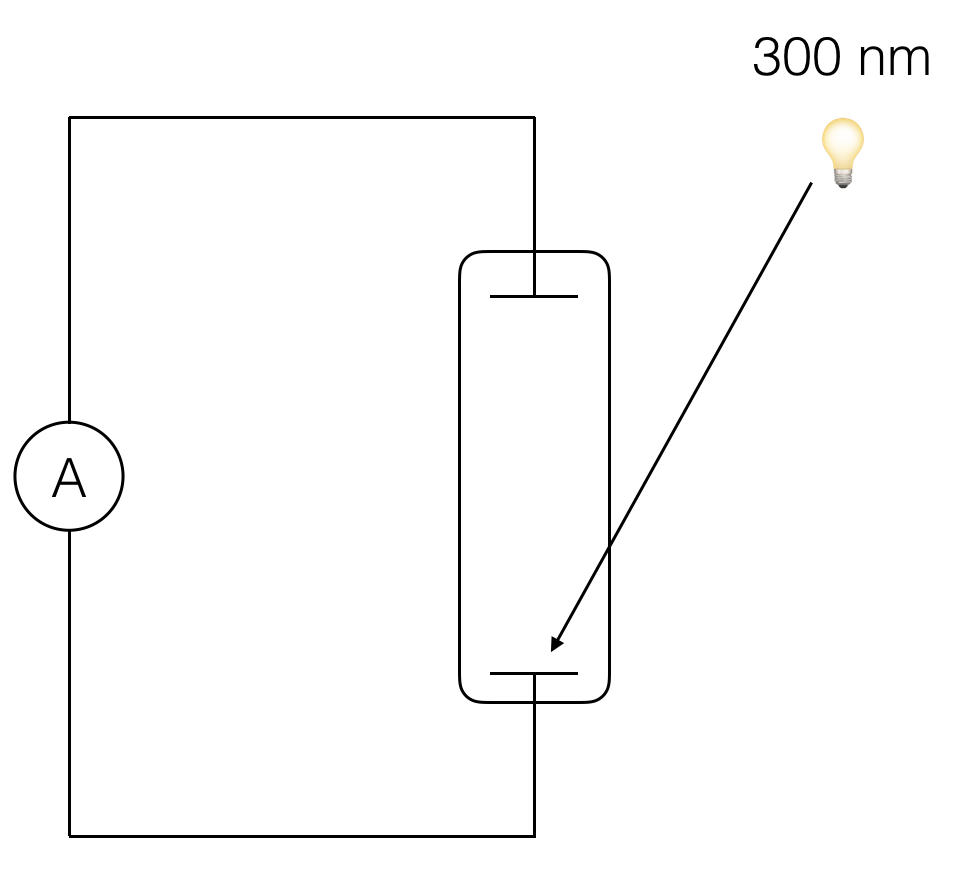
\includegraphics[width=0.45\textwidth]{../images/test2_300nm1.png}
\end{center}
	\begin{choices}
		\choice The two setups emit the same number of electrons, however the setup on the left emits electrons with greater energies.
		\choice The two setups emit the same number of electron, however the setup on the right emits electrons with greater energies.
		\choice The two setups emit electrons at the same energies, however the setup on the left emits more.
		\choice The two setups emit electrons at the same energies, however the setup on the right emits more.
		\choice The two setups emit the same number of electrons and at the same energies.
	\end{choices}
	\begin{TheSolution}
	\textbf{C.} Since light in both setups has the same wavelength, they transfer the same amount of energy to the electrons. However, since light on the left has a greater intensity it produces more photons and thus emits more electrons.
	\end{TheSolution}

\end{parts}
	
\clearpage
\question A nuclear physicist in a lab wishes to create oxygen. The graph below shows the binding energies for different elements and isotopes:
\noindent\begin{center}
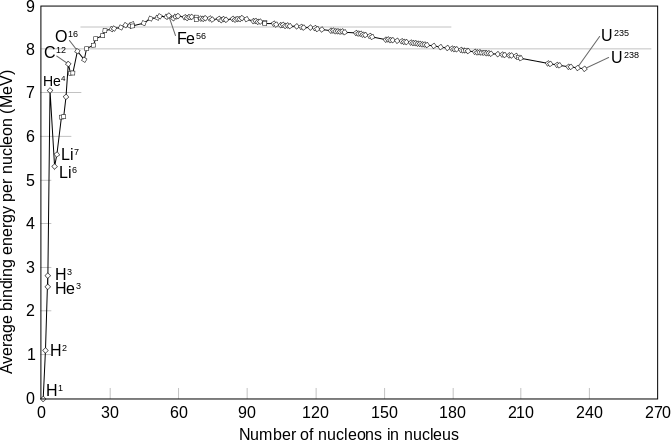
\includegraphics[width=0.9\textwidth]{../images/bindingEnergies.png}
\end{center}
\begin{parts}
	\part She combines $^3He$ to create $^{16}O$. Overall, would this release or require energy?
		\begin{TheSolution}
			It would \textbf{release} energy. The binding energy for oxygen-16 is greater than that for helium-3, meaning that it would take more energy to break apart oxygen than helium. Conversely, it would release more energy to form oxygen than helium, meaning that to combine helium from oxygen it would release energy.
		\end{TheSolution}
	\part She breaks apart $^{56}Fe$ to create $^{16}O$. Overall, would this release or require energy?
		\begin{TheSolution}
			It would \textbf{require} energy. The binding energy for iron-56 is greater than it is for oxygen-16.
		\end{TheSolution}
\end{parts}

\question $^{234}$Pu decays in two different ways:
\begin{enumerate}
	\item Via beta decay, where a neutron become a proton, and in the process emits an electron and an anti-neutrino:
	\begin{eqnarray}
	n \rightarrow p^+ + e^- + \bar{\nu} \nonumber
	\end{eqnarray}
	\item Via alpha decay, where a $^4$He nucleus is emitted.
\end{enumerate}
What are the two different isotopes created as products of these two modes of decay?

From \textit{Light and Matter}, Chapter 26 Question 3.
\begin{TheSolution}
\begin{enumerate}
	\item Through beta decay, $^{234}$Pu becomes Americium-234 ($^{234}$Am)
	\item Through alpha decay,  $^{234}$Pu becomes Uranium-230 ($^{230}$U)
\end{enumerate}
\end{TheSolution}

\question Suppose $^{244}$Pu undergoes a perfectly symmetric fission, and in the process emits 2 neutrons. What would be the two daughter nuclei? (Be sure to list the number of protons and neutrons in each).
\begin{TheSolution}
	\textbf{$^{121}$Ag} Each nucleus would have $94/2 = 47$ protons, and so would be silver (Ag). Each nucleus would have $\frac{244 - 94 - 2}{2} = 74$ neutrons, and so this would be silver-121
\end{TheSolution}

\question The masses of different particles are shown below:

\begin{tabular}{l l }
	proton & $1.67265 \times 10^{-27}$ kg \\
	electron & $0.00091 \times 10^{-27}$ kg \\
	neutron & $1.67495 \times 10^{-27}$ kg\\
	antineutrino & $< 10^{-35}$ kg
\end{tabular}

\begin{parts}
	\part Considering Einstein's equation which relates mass to energy via $E=mc^2$, which particle contains the greatest mass-energy?
		\begin{TheSolution}
			\textbf{Neutron} since it has the greatest mass.
		\end{TheSolution}
	\part Which particle contains the least mass-energy?
		\begin{TheSolution}
			\textbf{Antineutrino} since it has the least mass.
		\end{TheSolution}
	\part By the principle of wave-particle duality, we know that these different particles also have different wavelengths. Below are 4 different waves (not to scale, shown with decreasing wavelength), which represent the wavelengths of these different particles (assuming their velocities are negligible). Label them.
\end{parts}

\begin{center}
	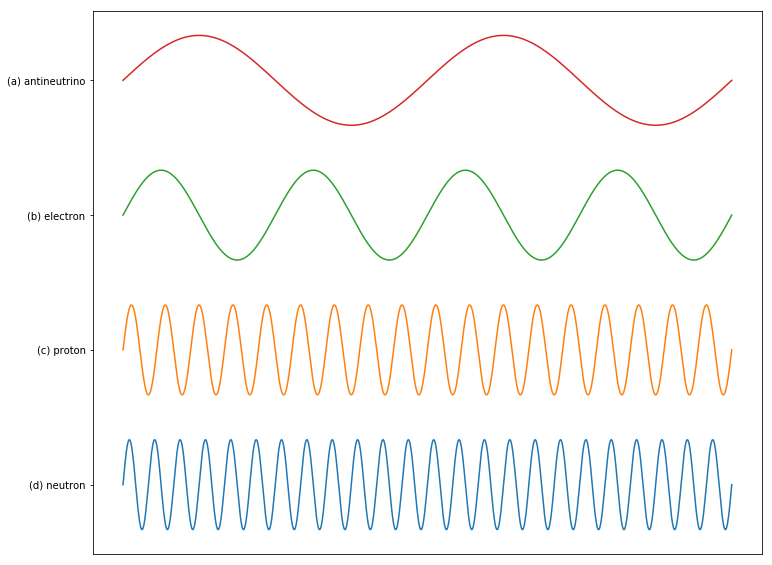
\includegraphics[width=0.9\textwidth]{../images/particleWavelengths_SOL.png}
\end{center}	

\question Suppose you have exactly 512 billion radioactive atoms, with a half-life of 10 hours.
	\begin{parts}
		\part How many atoms would you expect to have \textbf{decayed} after 10 hours?
			\begin{TheSolution}
				\textbf{256 Billion} 10 hours is 1 half-life, so you expect 1/2 to remain: therefore 1/2 to have decayed.
			\end{TheSolution}
		\part How many atoms would you expect to have \textbf{decayed} after 30 hours?	
			\begin{TheSolution}
				\textbf{448 Billion.} 30 hours is 3 half-lives, so you expect about $1/2 \times 1/2 \times 1/2 = 1/8$ to remain, which means $1 - 1/8 = 7/8$ to have decayed: $512~billion \times 7/8 = 448~billion$.
			\end{TheSolution}
		\part Suppose your friend also has exactly 512 billion radioactive atoms, also with a half-life of 10 hours. After 10 hours, how many atoms would they expect to have decayed after 10 hours?
			\begin{TheSolution}
				\textbf{256 Billion.} 10 hours is 1 half-life, so you expect 1/2 to remain: Therefore 1/2 to have decayed.
			\end{TheSolution}
		\part You and your friend count exactly how many atoms had decayed in 10 hours. Would these two numbers be exactly the same? \textbf{Explain.}
			\begin{TheSolution}
				\textbf{No} The odds of them being exactly the same are almost 0, just like if you flipped a coin 512 billion times and you friend did the same: you would expect to each get about 1/2 head and 1/2 tails, but not exactly the same number.
			\end{TheSolution}
	\end{parts}
	
\question The coating on the inside of fluorescent light tubes absorbs ultraviolet light and subsequently emits visible light. An inventor claims he is able to do the reverse process. Is the inventor's claim possible? (Think conservation laws...)
	\begin{TheSolution}
		\textbf{No.} When the coating on fluorescent light absorbs ultraviolet light and emits visible light, it's taking something with a lot of energy (UV light) and emitting something with less energy (visible light), and in the process some of this energy gets converted to heat (which is why the bulb gets hot). The inventor's claim would take something with very little energy (visible light) and then create something with much more light (UV light) which seems to create energy out of nothing - violating conservation of energy.
	\end{TheSolution}

\question Is the event horizon of a black hole the actual physical surface of the object?

From \textit{College Physics,} Chapter 34 Question 16.
\begin{TheSolution}
	\textbf{No} it the invisible boundary around the object beyond which light cannot escape due to the warping of spacetime: It's not a surface of the physical object, it's an invisible boundary in space.
\end{TheSolution}

\question Black holes are formed when the \textit{density} of an object becomes so large than space is warped to the point light cannot escape: This means there are very massive black holes (that are many times the mass of our sun) and very small black holes (that can have the mass of an asteroid, compressed to a space small enough). Suppose the moon were to be compressed to the point that it becomes a black hole - how would this effect life on Earth?
\begin{TheSolution}
	 \textbf{It would have almost no effect.} The mass stays the same, and so the gravitational pull would stay the same (the motion of the Earth and effect on the tides would stay the same). We would simply not notice the moon in the night sky, and instead would notice the effect of gravitational lensing on stars in the night sky as the moon/black hole orbited around the Earth.
\end{TheSolution}

\question Suppose we launch a satellite into a black hole. The satellite has on it a blinking light, which we are able to observe from our safe point very far away.

\input{../images/blackHoleProbe.pdf_tex}

\begin{parts}
	\part At which point (a), (b), (c), does the probe experience the strongest gravitational field?
		\begin{TheSolution}
			\textbf{(c)}  It is the closest to the black hole.
		\end{TheSolution}
	\part To an observer on Earth, what happens to the time between light flashes (from the blinking light) as the probe goes from (a) to (b) to (c)?
		\begin{TheSolution}
			\textbf{It increases.} As the probe falls into a stronger and stronger gravitational well, the time dilation becomes greater, meaning events appear to happens slower. Thus, the time between events (flashes) must take longer.
		\end{TheSolution}
	\part To an observer on Earth, what happens to the wavelength of the light in the light flashes as the probe goes from (a) to (b) to (c)?	
		\begin{TheSolution}
			\textbf{It Increases.} Since light will be coming from an increasingly stronger gravitational well, it will be more and more red-shifted: Thus the wavelength will be longer and longer.
		\end{TheSolution}
	\part What happens to the time between light flashes when the probe reaches the event horizon?
		\begin{TheSolution}
			The time gets longer and longer, and then becomes infinite (as though the probe freezes).
		\end{TheSolution}
	\part If someone were on the probe observing people on Earth, what would they see as they approach the event horizon?
		\begin{TheSolution}
			They would see light from the Earth getting more and more blue shifted, and then events happening faster and faster: They would be able to see the complete evolution of Earth's civilization, and watch as the universe ages to infinity.
		\end{TheSolution}
\end{parts}

\question Light from distant galaxies appears red-shifted, indicating that we are moving apart from each other. Furthermore, the further away an object the more red-shifted it is: Indicating that the universe is expanding. Explain (using the cosmological model of the evolution of the universe) why it only appears that we are at the center of expansion of the universe and why an observer in another galaxy would see the same relative motion in all but the closest galaxies away from her.

From \textit{College Physics}, Chapter 34 Conceptual Question 1.
\begin{TheSolution}
	Everything is moving away from everything else, like points on a balloon being inflated. Because of this, it doesn't matter where an observer is, they will still observe galaxies moving away from them.
\end{TheSolution}

\question In the beginning of this course, we discussed philosophy of science and the idea that scientific ideas must be falsifiable (meaning, it is possible to design an experiment that would disprove them). 

\begin{parts}
\part As light escapes a gravitational well, it is red-shifted. Galaxies are very massive objects, and have a gravitational field around them (which is why light bends around them). Therefore, if we observe light from a distant galaxy much more dense than our own, we would expect it to be red-shifted (since light would be moving from a large gravitational field to a relatively weaker one here on Earth).

Theoretically, we could use this to explain the redshift in light from distant galaxies, and could therefore disprove the theory that the universe is expanding. Propose an experiment/observation that could disprove this.
\begin{TheSolution}
We could look at the redshift of galaxies as a function of size/density, and see if the two are correlated.
\end{TheSolution}

\part Propose an experiment/observation that could test between these two theories: (1) Universe is expanding (2) Red-shift in light is due to gravitational fields of distant galaxies.

\begin{TheSolution}
	By plotting distance as a function of redshift, we can see that the more redshifted things are the further away the must be (or, conversely, the more distant things are the more redshifted they are):
	\begin{center}
	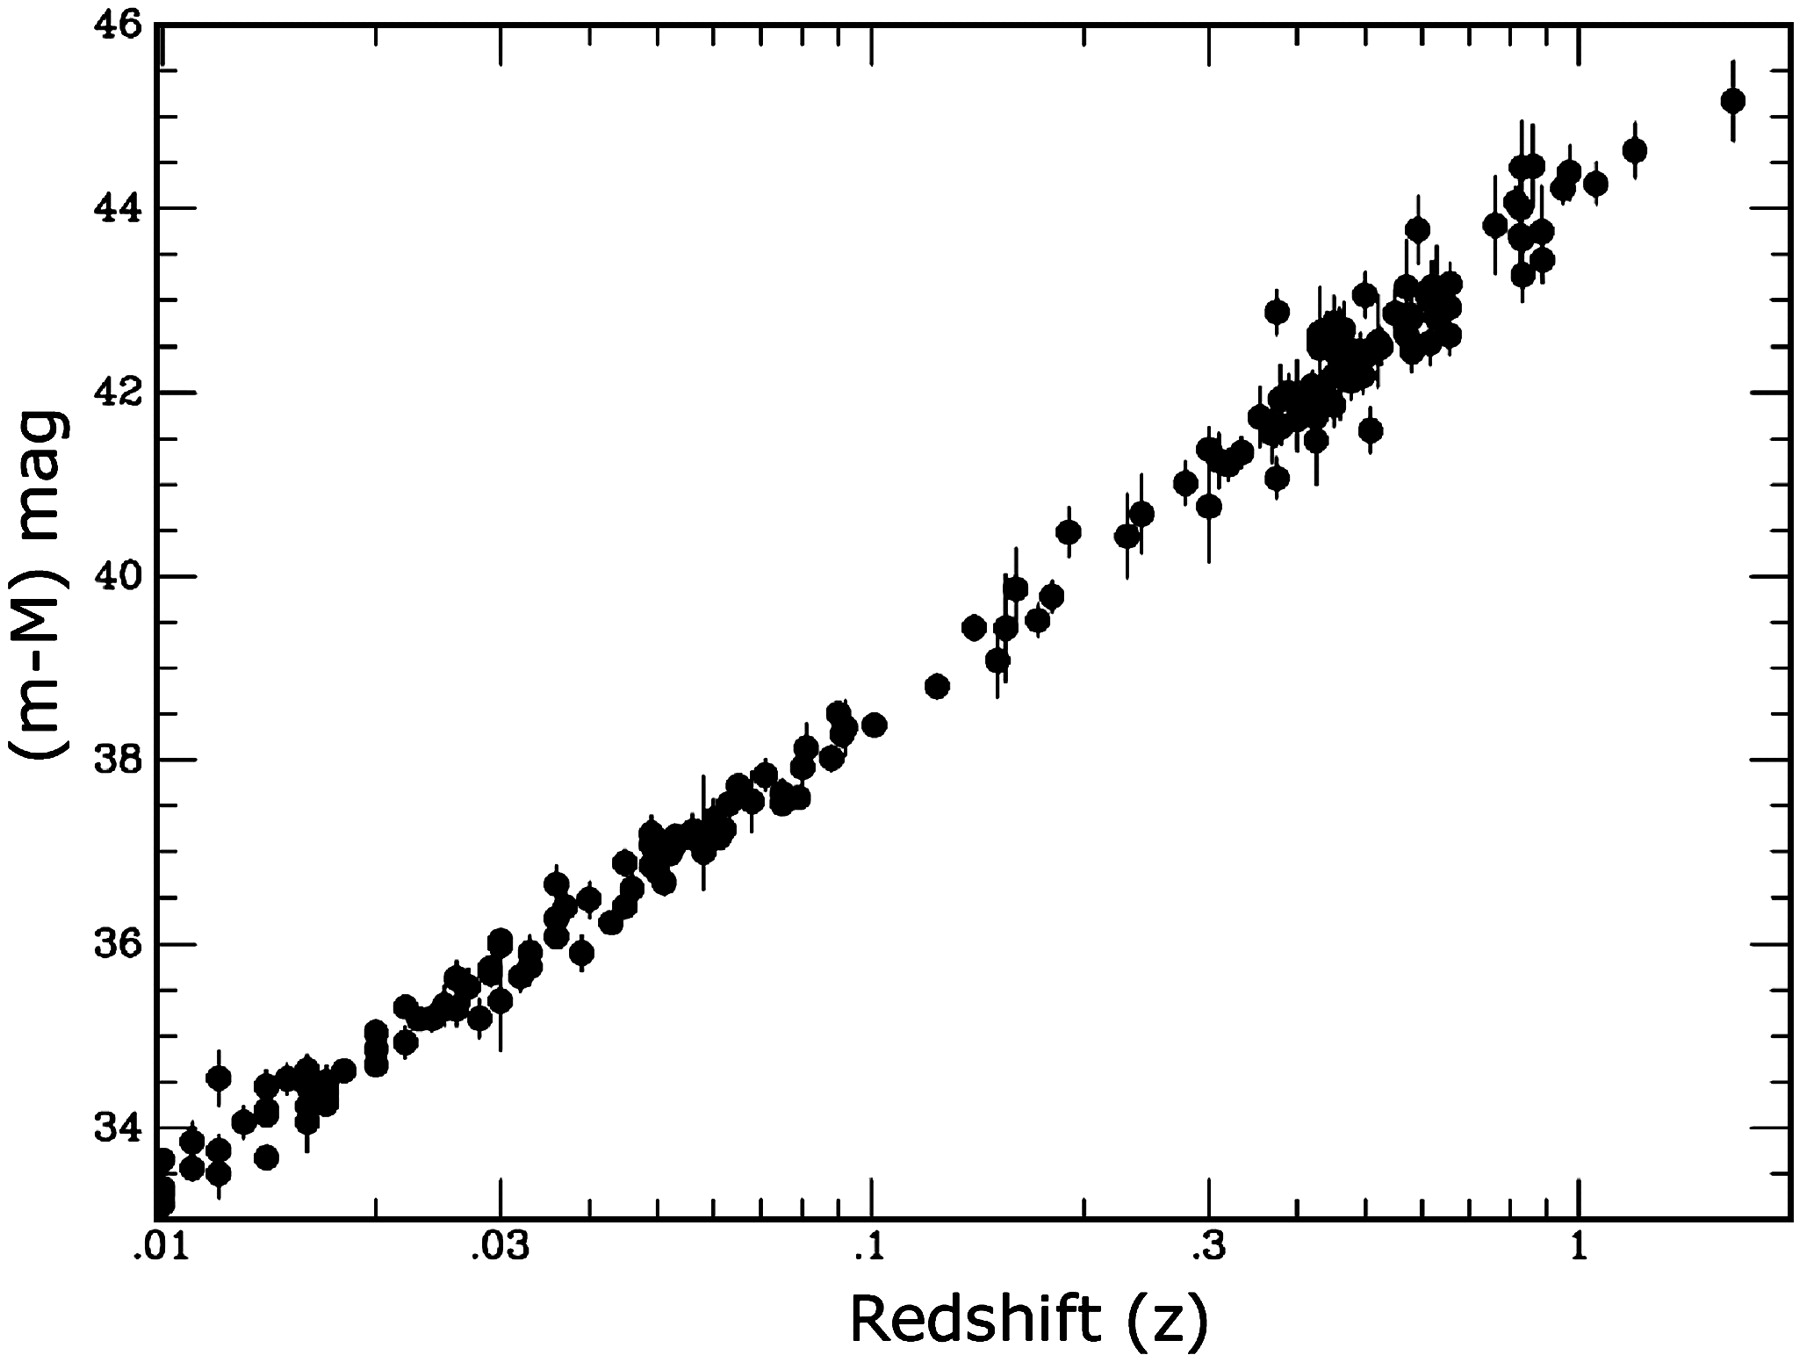
\includegraphics[width=0.5\textwidth]{../images/redshift.jpg}
	
	(image taken from R.P. Kirshner, \textit{Hubble's diagram and cosmic expansion}. PNAS \textbf{101(1)} 8-13 2004.)
	\end{center}
\end{TheSolution}
\end{parts}

\question Imagine you are walking through a forest. You know a tree is in front of you because you can see it (and you know this without needing to test further, say by reaching out and touching it) and so you walk around the tree so as to not walk into it. People who are visually impaired use canes to see, by sweeping the area in front of them. If the cane hits something, they feel the impact on the cane and know to avoid the object - in this way, someone who is blind knows there's a tree in front of them and will walk around it as well.
\begin{parts}
	\part Are these two ways of ``seeing" fundamentally different? Is using a tool to ``see" the world less valid than using our senses?
		\begin{TheSolution}
		There is no ``correct" answer to this question.
		\end{TheSolution}
	\part We cannot see individual atoms because we are too big, or distant black holes because we are so small. Instead, we rely on tools to probe for us (for atoms, we can look at the Brownian motion of microscopic particles and for black holes we can observe the effect they have on the orbits of stars surrounding them). Do you think this is a valid way to ``see" the universe, or is it too fundamentally different from seeing with our own senses to be comparable?
		\begin{TheSolution}
		There is no ``correct" answer to this question.
		\end{TheSolution}
\end{parts}

\question You have three fair, six-sided dice. You roll all three of them at once.
\begin{parts}
	\part What is the probability of rolling all 1s? P(1,1,1) = ?
		\begin{TheSolution} \textbf{About 0.5\% chance}
		
			There is only 1 way to roll 3 ones:
			\begin{eqnarray}
			P(1,1,1) = \frac{1}{6} \times \frac{1}{6} \times \frac{1}{6} = \frac{1}{216} \approx 0.0046
			\end{eqnarray}
		\end{TheSolution}
	\part What is the probability of rolling three of a kind? P(x,x,x) = ?
		\begin{TheSolution} \textbf{About 3\% chance}
		
		There are 6 ways to roll three of a kind, each with probability given in (a):
		\begin{eqnarray}
		& ~ & P(1,1,1)+ P(2,2,2) + P(3,3,3) + P (4,4,4) + P(5,5,5) + P(6,6,6) \\
		&=& \frac{1}{216} + \frac{1}{216} + \frac{1}{216} + \frac{1}{216} + \frac{1}{216} + \frac{1}{216} \\
		&=& \frac{6}{216} = \frac{1}{36} \approx 0.028
		\end{eqnarray}
		\end{TheSolution}
	\part What is the probability of rolling a one and two twos? P(1 and 2 and 2)
		\begin{TheSolution} \textbf{About 1\% chance}
			There are 3 ways to get this:
			\begin{eqnarray}
			P(1~and~2~and~2) &=& P(1,2,2) + P(2,1,2) + P(2,2,1) \\
			&=& \frac{1}{216} + \frac{1}{216} + \frac{1}{216} \\
			&=& \frac{3}{216} = \frac{1}{72} \approx 0.014
			\end{eqnarray}
		\end{TheSolution}
	\part What is the probability of rolling a one and two of a kind (that aren't ones)? 1,2,2 or 1,3,3 or 1,4,4 or 1,5,5 or 1,6,6
		\begin{TheSolution}\textbf{About 7\% chance}
		
		There are 5 different outcomes which satisfy this, each with a probability given in (c)
		\begin{eqnarray}
		&~& P(1~and~2~and~2) + P(1~and~3~and~3) + P(1~and~4~and~4) + P(1~and~5~and~5) \nonumber \\
		&~& + P(1~and~6~and~6) \\
		&=& \frac{1}{72} + \frac{1}{72} + \frac{1}{72} + \frac{1}{72} + \frac{1}{72} \\
		&=& \frac{5}{72} \approx 0.069
		\end{eqnarray}
		\end{TheSolution}
	\part What is the probability of rolling one, two and a three?
		\begin{TheSolution}\textbf{About 3\% chance}
		
			There are 6 different ways to get this, each with probability given in (a):
			\begin{eqnarray}
			&~& P(1,2,3) + P(1,3,2) + P(2,1,3) + P(2,3,1) + P(3,1,2) + P(3,2,1) \\
			&=& \frac{1}{216} +  \frac{1}{216} + \frac{1}{216} + \frac{1}{216} + \frac{1}{216} + \frac{1}{216}\\
			&=& \frac{6}{216} = \frac{1}{36} \approx 0.028
			\end{eqnarray}
		\end{TheSolution}
\end{parts}

\end{questions}

\end{document}
